% !TeX root = ../../../book.tex
\subsection{高斯驾到}\label{sec:section1.4.2}

\subsubsection*{问题描述}

数学界流传着一个关于史上最伟大数学家兼物理学家之一——卡尔·弗里德里希·高斯 (Carl Friedrich Gauss) 的著名轶事。无论故事真实与否,其魅力令无数人深信不疑。高斯活跃于 18 世纪末至 19 世纪中叶,在数论、复分析、光学、几何学及天文学等诸多领域做出了奠基性贡献。请阅读下面这则故事,设想自己(无论童年或现在)会如何应对,然后再继续探讨。

\begin{quote}
    清晨,小学教室里喧闹的学生令老师不胜其烦。为获得片刻安宁,他急需让学生们专注做事。老师高声要求学生取出石板和粉笔。待众人准备就绪,他布置了一道题目:计算从 $1$ 到 $100$ 所有整数之和,并承诺最先完成者可担任当日助教。老师回到座位,料想繁重的计算将让学生们安静许久。不料仅过一分钟,一个男孩便带着写有答案的石板前来。老师惊讶之余亲自验算,结果证实男孩答案完全正确。他是如何快速完成计算的?
\end{quote}

请认真思考后再翻阅解答。请注意:这则故事``发生''在计算器尚未问世的年代,解题只能依靠纸笔与心算能力。

\clearpage

\subsubsection*{解答:简化计算}

也许你已经找到了窍门。实际上,这个问题有多种解法,它们大多基于相同的核心思路:尽量减少所需的计算量。

如果简单地遍历这 $100$ 个数字并逐个累加,需要进行 $99$ 次加法,且运算数字会越来越大。当然,技巧不仅仅在于更快地执行加法,而在于从根本上提高计算效率。我们知道,乘法本质上是数字与其自身的重复加法。因此,如果能找到合适的数字进行重复自加,就有可能将大量加法简化为一次乘法。

另一个关键点是加法满足\textbf{结合律}和\textbf{交换律},这意味着加法的顺序不影响最终结果。具体而言,无论将数字从 $1$ 加到 $100$ 还是从 $100$ 加到 $1$,其总和 $S$ 都相同。我们可以这样表示:
\begin{center}
    \begin{tabular}{ccccccccccccccc}
          1 & + &   2 & + &   3 & + & \dots & + &  98 & + &  99 & + & 100 & = & S\\\noalign{\smallskip\smallskip}
        100 & + &  99 & + &  97 & + & \dots & + &   3 & + &   2 & + &   1 & = & S\\\noalign{\smallskip\smallskip}
        \hline
        101 & + & 101 & + & 101 & + & \dots & + & 101 & + & 101 & + & 101 & = & 2S\\\noalign{\smallskip\smallskip}
    \end{tabular}
\end{center}
注意,我们以两种顺序写出了总和 $S$。将这两个等式逐项相加,得到总和 $2S$ 的表达式。这个新表达式可直接转换为乘法,因为有 $100$ 项,每项都等于 $101$。因此:
\begin{align*}
    2S &= 101 \cdot 100 \\
     S &= 101 \cdot 50 = 5050
\end{align*}
这比执行 $99$ 次加法要快得多。事实上,只要稍加练习,我们完全能在脑海中完成整个计算过程!

\subsubsection*{另一种解法:配对法}

解决该问题的相似思路是省去两行相加的中间步骤,直接将原始求和中的数字配对,如下所示:
\begin{align*}
    S &= 1 + 2 + 3 + \dots + 98 + 99 + 100 \\
    &= (1 + 100) + (2 + 99) + (3 + 98) + \dots + (49 + 52) + (50 + 51) \\
    &= 101 + 101 + \dots + 101 = 50 \cdot 101 = 5050
\end{align*}
该方法与前述解法本质相同,均利用加法交换律和结合律重组求和项,只是跳过了求 $2S$ 表达式然后再除以 $2$ 这一中间步骤。

\subsubsection*{泛化:$n$ 为偶数}

如果老师要求学生计算 $1$ 到 $1000$ 的数字之和呢?学生是否会抗议?高斯能否同样迅速作答?我们虽不确定前两个问题的答案,但相信你一定能轻松解决。这里唯一不同的是,我们需要创建 $500$ 组配对(而非 $50$ 组),每组之和为 $1001$(而非 $101$),因此结果为
\[1 + 2 + 3 + \dots + 998 + 999 + 1000 = 1001 \cdot 500 = 500500\]

看起来是不是存在某种规律呢?你觉得你能在不进行乘法的情况下立即说出 $1$ 到 $100$ 万之间所有数字之和是多少吗?

\subsubsection*{泛化:$n$ 为奇数}

如果老师要求的是前 $99$ 个数字之和呢?配对法是否仍然适用?让我们验证一下:
\begin{align*}
    S &= 1 + 2 + 3 + \dots + 97 + 98 + 99 \\
    &= (1 + 99) + (2 + 98) + (3 + 97) + \dots + (48 + 52) + (49 + 51) + 50 \\
    &= (49 \cdot 100) + 50 = 4950
\end{align*}
请注意,总项数为奇数,因此无法将所有数字完全配对,必须在乘法结果上加上中间项 $50$。是否有其他配对方式?
\begin{align*}
    S &= 1 + 2 + 3 + \dots + 97 + 98 + 99 \\
    &= (1 + 98) + (2 + 97) + (3 + 96) + \dots + (48 + 51) + (49 + 50) + 99 \\
    &= (49 \cdot 99) + 99 = 50 \cdot 99 = 4950
\end{align*}
这种方法\emph{看起来}与原始谜题的结果更相似,因为我们只执行\emph{一次}乘法。这是巧合吗?请尝试用相同方法计算其他奇数项之和:前 $7$ 个整数之和是多少?前 $29$ 个呢?前 $999$ 个呢?前 $999999$ 个呢?

\subsubsection*{泛化:任意 $n$}

让我们从个案研究中抽离出来,尝试从更一般的视角解决这个问题。假设老师向学生提出了以下问题:
\begin{quote}
    给出前 $n$ 个自然数之和的公式。我需要一个具体的公式,这样当有人告诉我 $n$ 的值时,我就能直接代入并快速得到答案。
\end{quote}

第二句的说明排除了其他方法。虽然我们之前提出过一些简单算法,但现在被要求给出一个直接计算的公式。该如何入手呢?根据之前的观察,分情况讨论 $n$ 的奇偶性是一个合理的策略。我们发现奇偶情况下的配对结果略有差异,因此先讨论其中一种情况,再讨论另一种。在每种情况下,我们都寻求 $S(n) = 1 + 2 + 3 + \dots + (n - 2) + (n - 1) + n$ 的表达式。这里用 $S(n)$ 表示这个和依赖于 $n$ 的值。

如果 $n$ 为偶数,我们可以将所有数完美配对:
\begin{align*}
    S(n) &= 1 + 2 + 3 + \dots + \left(\frac{n}{2}-1\right) + \frac{n}{2} + \left(\frac{n}{2}+1\right) + \dots + (n - 2) + (n - 1) + n\\
    &=  (1 + n) + \left(2 + (n - 1)\right) + \left(3 + (n - 2)\right) + \dots + \left(\left(\frac{n}{2}-1\right)+\left(\frac{n}{2}+2\right)\right) + \left(\frac{n}{2}+\left(\frac{n}{2}+1\right)\right) \\
    &= (n+1)\frac{n}{2} = \frac{n^2+n}{2}
\end{align*}

将已知结果的偶数(如 $n=100, 1000, 1000000$)代入公式进行验证。注意,公式中出现 $\frac{n}{2}$ 是合理的,因为 $n$ 为偶数,$\frac{n}{2}$ 必为整数。

如果 $n$ 为奇数呢?此时无法将所有数完全配对,需要巧妙处理。回想前 $99$ 项求和的方法,通过暂时忽略末项 $n$,将剩余项配对。有趣的是,每对之和恰好等于末项 $n$。让我们尝试运用此方法:
\begin{align*}
    S(n) &= 1 + 2 + 3 + \dots + \left(\frac{n-1}{2}-1\right) + \frac{n-1}{2} + \left(\frac{n-1}{2}+1\right) + \dots + (n - 2) + (n - 1) + n\\
    &=  \left(1 + (n-1)\right) + \left(2 + (n - 2)\right) + \dots + \left(\left(\frac{n-1}{2}\right)+\left(\frac{n-1}{2}+1\right)\right) + n \\
    &= n+n+ \dots + \left(\frac{2n-2}{2}+1\right) +n = (n+n+\dots+n)+n
\end{align*}

这表明每对数字之和为 $n$,即我们最初忽略的末项。现在计算配对数量:第一对是 $(1, n - 1)$,第二对是 $(2, n - 2)$,依此类推,最后一对的首项为 $\frac{n-1}{2}$。因此共有 $\frac{n-1}{2}$ 对。(注意 $n$ 为奇数保证了 $n-1$ 为偶数,故 $\frac{n-1}{2}$ 为整数。请回顾推导过程,确认每一步的有效性。)加上末项 $n$,总和可表示为:
\[S(n) = \left(\frac{n-1}{2} + 1\right) \cdot n = \left(\frac{n-1}{2} + \frac{2}{2}\right) \cdot n = \frac{n+1}{2} \cdot n = \frac{n^2+n}{2}\] 

令人惊讶的是,这与 $n$ 为偶数时得到的公式完全相同!你是否感到意外?虽然奇偶情况的解法相似,但并无明显迹象预示结果会一致。这对我们有什么启示?数学家面对这种``巧合''时,会思考是否存在\emph{更简洁}、\emph{更普适}的解法——能否用一种方法同时处理奇数和偶数\emph{两种}情况?既然结果相同,这样的方法很可能存在。请在继续阅读前先思考一下这个问题。

\subsubsection*{泛化:任意 $n$, \emph{不}分开讨论}

事实证明,我们在之前讨论这道谜题时已经暗示过另一种方法。还记得将正序求和写在一行、倒序求和写在另一行并将它们相加吗?当时处理奇偶性问题时,我们因看似步骤繁琐而避开了此法;``配对法''似乎更快捷,所以我们便采用了配对法。但若重新审视``两次相加''这一方法,会得到什么?我们会发现:
\begin{center}
    \begin{tabular}{ccccccccccc}
           1  & + &     2 & + & \dots & + & (n-1) & + &     n & = & S(n)\\\noalign{\smallskip\smallskip}
           n  & + & (n-1) & + & \dots & + &     2 & + &     1 & = & S(n)\\\noalign{\smallskip\smallskip}
        \hline
        (n+1) & + & (n+1) & + & \dots & + & (n+1) & + & (n+1) & = & 2S(n)\\\noalign{\smallskip\smallskip}
    \end{tabular}
\end{center}
此时第三行求和包含 $n$ 项,每项均为 $(n + 1)$。因此:
\begin{align*}
    2S &= (n+1) \cdot n \\
     S &= \frac{1}{2}(n+1) \cdot n = \frac{n^2+n}{2}
\end{align*}
这正是此前推导的公式,而此处的推导过程完全不依赖 $n$ 的奇偶性!(请回顾上述步骤并自行验证 $n$ 的奇偶性确实无关紧要。)

\subsubsection*{第三种解法:可视化图表}

在结束此问题之前,我们介绍一种几何解法。我们将求和 $S(n)$ 与正方形的面积关联,并将求和的各项($1, 2, 3, \dots, n - 1, n$)可视化为正方形的一部分。具体来说,考虑一个 $n \times n$ 的正方形,并将各项表示为宽度为一个单位、高度递增的矩形。见下图:

\begin{center}
    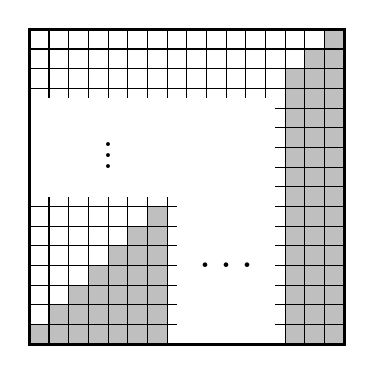
\begin{tikzpicture}[scale=0.5, x=0.5cm, y=0.5cm, font=\LARGE]
        \foreach \x in {0,...,15} 
            \foreach \y in {0,...,15}
                {
                    \pgfmathparse{(\x >= \y && (\x<7 || \x>12)) ? "lightgray" : "white"}
                    \edef\colour{\pgfmathresult}
                    \path[fill=\colour] (\x,\y) rectangle ++ (1,1);
                    \draw[black] (\x,\y) rectangle ++ (1,1);
                }
        \fill[white] (0, 7.5) rectangle ++ (8,5) node[color=black, pos=.5, align=center]{$\vdots$};
        \fill[white] (7.5, 0) rectangle ++ (5,8) node[color=black, pos=.5, align=center]{$\dots$};
        \fill[white] (7.5, 7.5) rectangle ++ (5,5) node[color=black, pos=.5, align=center]{$\iddots$};
        \draw[very thick, black] (0, 0) rectangle ++ (16,16);
    \end{tikzpicture}
\end{center}

现在,要求 $S(n)$ 的公式等价于计算正方形内所有矩形覆盖的\emph{面积}。直接相加各矩形面积只是重复原问题,因此我们需要将该面积与正方形的总面积关联。为此,考虑剩余区域,如何描述未被矩形覆盖的部分?观察第一个 $1 \times 1$ 矩形正上方的区域:它是一个尺寸为 $(n - 1) \times 1$ 的矩形。

类似地,$2 \times 1$ 矩形上方的区域是一个 $(n-2) \times 1$ 矩形。此模式持续下去!最终,在 $(n - 1) \times 1$ 矩形上方为一个 $1 \times 1$ 矩形,而最后一个 $n \times 1$ 矩形上方无区域。这些矩形的总面积类似于 $S(n)$,但缺少最后一项 $n$。现在,将所有矩形的面积与 $S(n)$ 和正方形面积关联:
\[n^2 = S(n) + (S(n) - n) = 2S(n) - n\]
解得
\[S(n) = \frac{n^2+n}{2}\]
与我们之前得到的公式一致!

\subsubsection*{解题心得}

有时,问题有多种解法。有些方法易于构思但难于求解;有些难以想到但求解简洁;还有些可能根本无效!通常无法预判哪种方法有效,因此建议动手尝试并观察结果。记录尝试的过程和结果,以便后续重新评估。这是数学学习中需牢记的原则:我们并非总能立即知晓正确路径,偶尔会陷入困境或走入死胡同。这不应令人沮丧;它是学习的一部分。

作为练习,尝试为 $n$ 为奇数的情况重新``配对'',不忽略求和的最后一项,而是分离中间项并将数字从外向内配对。这会得到相同结果吗?该方法是否比原解法更简便、更快速或有所不同呢?或者,对于 $n$ 为偶数的情况,令 $n=2k$ 会怎样?对于 $n$ 为奇数又该如何操作?这种表示会改变处理过程吗?会使问题更容易处理吗?现在,你能构思一种全新的解法吗?
